%
% This is the LaTeX template file for lecture notes for CS294-8,
% Computational Biology for Computer Scientists.  When preparing 
% LaTeX notes for this class, please use this template.
%
% To familiarize yourself with this template, the body contains
% some examples of its use.  Look them over.  Then you can
% run LaTeX on this file.  After you have LaTeXed this file then
% you can look over the result either by printing it out with
% dvips or using xdvi.
%
% This template is based on the template for Prof. Sinclair's CS 270.

\documentclass[twoside]{article}
\usepackage{graphics}
\usepackage{amsmath}
\usepackage{amssymb}
\usepackage{hyperref}
\usepackage{IEEEtrantools}
\usepackage{graphicx}
\usepackage{float}
\usepackage{listings}

\setlength{\oddsidemargin}{0.25 in}
\setlength{\evensidemargin}{-0.25 in}
\setlength{\topmargin}{-0.6 in}
\setlength{\textwidth}{6.5 in}
\setlength{\textheight}{8.5 in}
\setlength{\headsep}{0.75 in}
\setlength{\parindent}{0 in}
\setlength{\parskip}{0.1 in}
\usepackage[makeroom]{cancel}
%
% The following commands set up the lecnum (lecture number)
% counter and make various numbering schemes work relative
% to the lecture number.
%
\newcounter{lecnum}
\renewcommand{\thepage}{\thelecnum-\arabic{page}}
\renewcommand{\thesection}{\thelecnum.\arabic{section}}
\renewcommand{\theequation}{\thelecnum.\arabic{equation}}
\renewcommand{\thefigure}{\thelecnum.\arabic{figure}}
\renewcommand{\thetable}{\thelecnum.\arabic{table}}

%
% The following macro is used to generate the header.
%
\newcommand{\lecture}[5]{
   \pagestyle{myheadings}
   \thispagestyle{plain}
   \newpage
   \setcounter{lecnum}{#1}
   \setcounter{page}{1}
   \noindent
   \begin{center}
   \framebox{
      \vbox{\vspace{2mm}
    \hbox to 6.28in { {\bf CMPUT 652: Reinforcement Learning with Robots
                        \hfill Fall 2019} }
       \vspace{4mm}
       \hbox to 6.28in { {\Large \hfill Lecture #1: #2  \hfill} }
       \vspace{2mm}
       \hbox to 6.28in { {\it Instructor: #3 \hfill Scribe: #4} }
      \vspace{2mm}}
   }
   \end{center}
   \markboth{Lecture #1: #2}{Lecture #1: #2}
   {\bf Disclaimer}: {\it These notes have not been subjected to the
   usual scrutiny reserved for formal publications.  They may be distributed
   outside this class only with the permission of the Instructor.}
   \vspace*{4mm}
}

%
% Convention for citations is authors' initials followed by the year.
% For example, to cite a paper by Leighton and Maggs you would type
% \cite{LM89}, and to cite a paper by Strassen you would type \cite{S69}.
% (To avoid bibliography problems, for now we redefine the \cite command.)
% Also commands that create a suitable format for the reference list.

%% This has been commented by Dhawal
% \renewcommand{\cite}[1]{[#1]}
% \def\beginrefs{\begin{list}%
%         {[\arabic{equation}]}{\usecounter{equation}
%          \setlength{\leftmargin}{2.0truecm}\setlength{\labelsep}{0.4truecm}%
%          \setlength{\labelwidth}{1.6truecm}}}
% \def\endrefs{\end{list}}
% \def\bibentry#1{\item[\hbox{[#1]}]}

%Use this command for a figure; it puts a figure in wherever you want it.
%usage: \fig{NUMBER}{SPACE-IN-INCHES}{CAPTION}
\newcommand{\fig}[3]{
			\vspace{#2}
			\begin{center}
			Figure \thelecnum.#1:~#3
			\end{center}
	}
% Use these for theorems, lemmas, proofs, etc.
\newtheorem{theorem}{Theorem}[lecnum]
\newtheorem{lemma}[theorem]{Lemma}
\newtheorem{proposition}[theorem]{Proposition}
\newtheorem{claim}[theorem]{Claim}
\newtheorem{corollary}[theorem]{Corollary}
\newtheorem{definition}[theorem]{Definition}
\newenvironment{proof}{{\bf Proof:}}{\hfill\rule{2mm}{2mm}}

% **** IF YOU WANT TO DEFINE ADDITIONAL MACROS FOR YOURSELF, PUT THEM HERE:

%%===========================================================================
%% defining the expectation operator
%%---------------------------------------------------------------------------
\newcommand{\vpi}{\mathbf{v}_{\pi}}
\newcommand{\rpi}{\mathbf{r}_{\pi}}
\newcommand{\Ppi}{\mathbf{P}_{\pi}}

% \DeclareMathOperator{\thetagd}{\theta^{GD}}
% \DeclareMathOperator{\rv}{X} % define random variable 
% \DeclareMathOperator{\sc}{} %
% \DeclareMathOperator{}{} %
% \DeclareMathOperator{}{} %
% \DeclareMathOperator{}{} %

% \DeclareMathOperator{}{}
%%===========================================================================

\begin{document}
%FILL IN THE RIGHT INFO.
%\lecture{**LECTURE-NUMBER**}{**DATE**}{**LECTURER**}{**SCRIBE**}
\lecture{8}{September 26}{Rupam Mahmood}{Kris De Asis}

% **** YOUR NOTES GO HERE:

% Some general latex examples and examples making use of the
% macros follow.  
%**** IN GENERAL, BE BRIEF. LONG SCRIBE NOTES, NO MATTER HOW WELL WRITTEN,
%**** ARE NEVER READ BY ANYBODY.

\section{Bellman Equation in Matrix Form}

Recall the Bellman equation for $v_{\pi}$:
\begin{equation}
    v_{\pi}(s) = \sum_{a}{\pi(a|s)\sum_{s',r}{p(s',r|s,a)\big(r + \gamma v_{\pi}(s')\big)}}
    \label{eqn:vbellman}
\end{equation}
We can separate the immediate reward from the remainder of the return:
\begin{equation*}
    v_{\pi}(s) = \sum_{a}{\pi(a|s)\sum_{s',r}{p(s',r|s,a)r}} + \gamma\sum_{a}{\pi(a|s)\sum_{s',r}{p(s',r|s,a)v_{\pi}(s')}}
\end{equation*}
Denoting $r(s,a) = \sum_{s',r}{p(s',r|s,a)r}$ and $p(s'|s, a) = \sum_{r}{p(s',r|s,a)}$, we get:
\begin{align}
    \nonumber
    v_{\pi}(s) &= \sum_{a}{\pi(a|s)r(s,a)} + \gamma\sum_{s'}{\Big[\sum_{a}{\pi(a|s)p(s'|s,a)}\Big]v_{\pi}(s')} \\
    v_{\pi}(s) &= r_{\pi}(s) + \gamma \sum_{s'}{p_{\pi}(s'|s)v_{\pi}(s')}
\end{align}
where $r_{\pi}(s) = \sum_{a}{\pi(a|s)r(s,a)}$ and $p_{\pi}(s'|s) = \sum_{a}{\pi(a|s)p(s'|s,a)}$. From here, we can write the Bellman equation in matrix form:
\begin{equation*}
    \begin{bmatrix}
        v_{\pi}(s_0) \\
        v_{\pi}(s_1) \\
        \vdots
    \end{bmatrix}
    =
    \begin{bmatrix}
        r_{\pi}(s_0) \\
        r_{\pi}(s_1) \\
        \vdots
    \end{bmatrix}
    + \gamma
    \begin{bmatrix}
        p_{\pi}(s_0|s_0) & p_{\pi}(s_1|s_0) & \dots \\
        p_{\pi}(s_0|s_1) & p_{\pi}(s_1|s_1) & \dots \\
        \vdots & \vdots & \ddots
    \end{bmatrix}
    \begin{bmatrix}
        v_{\pi}(s_0) \\
        v_{\pi}(s_1) \\
        \vdots
    \end{bmatrix}
\end{equation*}
\begin{equation}
    \vpi = \rpi + \gamma \Ppi \vpi
    \label{eqn:vbmat}
\end{equation}

\section{Policy Evaluation}
Value functions provide a way of valuating policies such that we can say whether one policy is better than another. Based on this, the process of computing a policy's value function is referred to as \textit{policy evaluation}. Here, we'll detail how we can use the Bellman equation to compute value functions.
An observation is that the Bellman equation produces a linear system of equations, which can be written in the form $\mathbf{A}\vpi = \mathbf{b}$:
\begin{align}
    \nonumber
    \vpi = \rpi + \gamma \Ppi \vpi \\
    \nonumber
    \vpi - \gamma \Ppi \vpi = \rpi \\
    \nonumber
    (\mathbf{I} - \gamma \Ppi) \vpi = \rpi
\end{align}
where $\mathbf{A} = \mathbf{I} - \gamma \Ppi$ and $\mathbf{b} = \rpi$. Based on this, we can solve the linear system with:
\begin{align}
    \nonumber
    \vpi &= \mathbf{A}^{-1}\mathbf{b} \\
    \vpi &= (\mathbf{I} - \gamma \Ppi)^{-1} \rpi
\end{align}
if $\mathbf{I} - \gamma \Ppi$ is invertible. Because $\Ppi$ is a stochastic matrix, the largest absolute value of its eigenvalues is 1. As it is being discounted and subtracted from the identity matrix, the real components of its eigenvalues should be positive, and its inverse exists. We can also solve the system iteratively:
\begin{equation}
    \mathbf{v}_{k+1} \leftarrow \mathbf{v}_{k} - \alpha (\mathbf{A} \mathbf{v}_{k} - \mathbf{b})
\end{equation}
where $\mathbf{v}_k$ converges to $\vpi$ as $k\rightarrow\infty$ (under some stochastic approximation conditions). Of note, $\alpha = 1$ corresponds to evaluating the Bellman equation for each state simultaneously using the current estimates:
\begin{align}
\nonumber
    \mathbf{v}_{k+1} &\leftarrow \mathbf{v}_{k} - (\mathbf{A} \mathbf{v}_{k} - \mathbf{b}) \\
    \nonumber
    \mathbf{v}_{k+1} &\leftarrow \mathbf{v}_{k} - \big((\mathbf{I} - \gamma \Ppi) \mathbf{v}_{k} - \rpi\big) \\
    \nonumber
    \mathbf{v}_{k+1} &\leftarrow \mathbf{v}_{k} - (\mathbf{v}_{k} - \gamma \Ppi \mathbf{v}_{k}  - \rpi) \\
    \nonumber
    \mathbf{v}_{k+1} &\leftarrow \rpi + \gamma \Ppi \mathbf{v}_{k}
\end{align}
A key limitation of these approaches are that they require a model of the world. That is, they need complete specification of the environment's rewards to get $\rpi$, as well as the state-transition dynamics for $\Ppi$.

\section{Policy Iteration}

Policy iteration is a process which allows for identifying the optimal policy. It relies on the policy improvement theorem, where producing a new policy that is greedy with respect to the values of the previous policy will result in a policy that is at least as good as the previous. If the new policy does not change after greedifying with respect to the values of the previous policy, then it is an optimal policy.

We denote a greedy-policy operator $g$, which produces a policy that is greedy with respect to the values of another policy:
\begin{equation*}
    g q_{\pi_{k}} = \pi_{k+1}
\end{equation*}
Starting with some initial policy $\pi_0$, policy iteration interleaves policy evaluation and policy improvement until the policy stops changing (and is optimal):
\begin{equation*}
    \pi_0 \rightarrow q_{\pi_0} \rightarrow g q_{\pi_0} \rightarrow  q_{\pi_1} \rightarrow g q_{\pi_1} \rightarrow q_{\pi_2} \rightarrow \dots \rightarrow \pi^*.
\end{equation*}

\section{Value Iteration}

Knowing that an optimal policy is one which is greedy with respect to the optimal value function, another approach is to evaluate the Bellman optimality equation. Considering action values, we have the following Bellman optimality equation:
\begin{align}
    \nonumber
    q_*(s,a) = \sum_{s',r}{p(s',r|s,a)\big(r + \gamma \max_{a'}{q_*(s',a')}\big)} \\
    \nonumber
    q_*(s,a) = r(s,a) + \gamma \sum_{s'}{p(s'|s,a)\max_{a'}{q_*(s',a')}}
\end{align}
Which can similarly be written in matrix form:
\begin{equation}
    \mathbf{q}_* = \mathbf{r} + \gamma \mathbf{P}_* \mathbf{q}_*
\end{equation}
Of note, the rows now correspond to every state-action pair of the MDP, and the $\mathbf{P}_*$ matrix maps state-action pairs to state-action pairs. Because the first action is specified, the policy determines the next state-action pair in the transition.

Because the policy now depends on the action-values, we have a non-linear system of equations and can't directly solve it with a matrix inverse. We'll have to resort to an iterative approach where at each iteration, the policy (implicitly represented through $\mathbf{P}$) is greedified with respect to the current values.
\begin{align}
    \nonumber
    \mathbf{q}_{k+1} &\leftarrow \mathbf{q}_{k} - \alpha(\mathbf{A}_{g\mathbf{q}_k}\mathbf{q}_k - \mathbf{b}) \\
    \mathbf{q}_{k+1} &\leftarrow \mathbf{q}_{k} - \alpha\big((\mathbf{I} - \gamma \mathbf{P}_{g \mathbf{q}_k})\mathbf{q}_k - \mathbf{r}\big)
\end{align}
This can be viewed as interleaving policy evaluation and policy improvement at a finer-grained level, where policy improvement is performed after each step of an iterative approach to policy evaluation. Once the values stop changing, the optimal value function has been found and an optimal policy can be inferred by greedifying with respect to it. This process of iteratively solving the Bellman optimality equation is referred to as \textit{value-iteration}.

\section{Unifying Continuing and Episodic Tasks}

Reinforcement learning tasks are typically categorized as one of two kinds of tasks: \textit{Episodic} tasks, where the underlying MDP has terminal (or absorbing) states, and \textit{continuing} tasks, where it does not. A reason for this distinction lies in that episodic returns are finite and can be undiscounted, while continuing tasks often rely on discounting (or some other reward transform) to ensure the infinite sum of rewards is well defined.

However, episodic tasks can also be framed as a continuing task if we allow the discount rate to vary on a state-dependent basis. Consider the undiscounted MDP specifying an episodic task in Figure \ref{fig:mdp_episodic}.

\begin{figure}[!h]
    \centering
    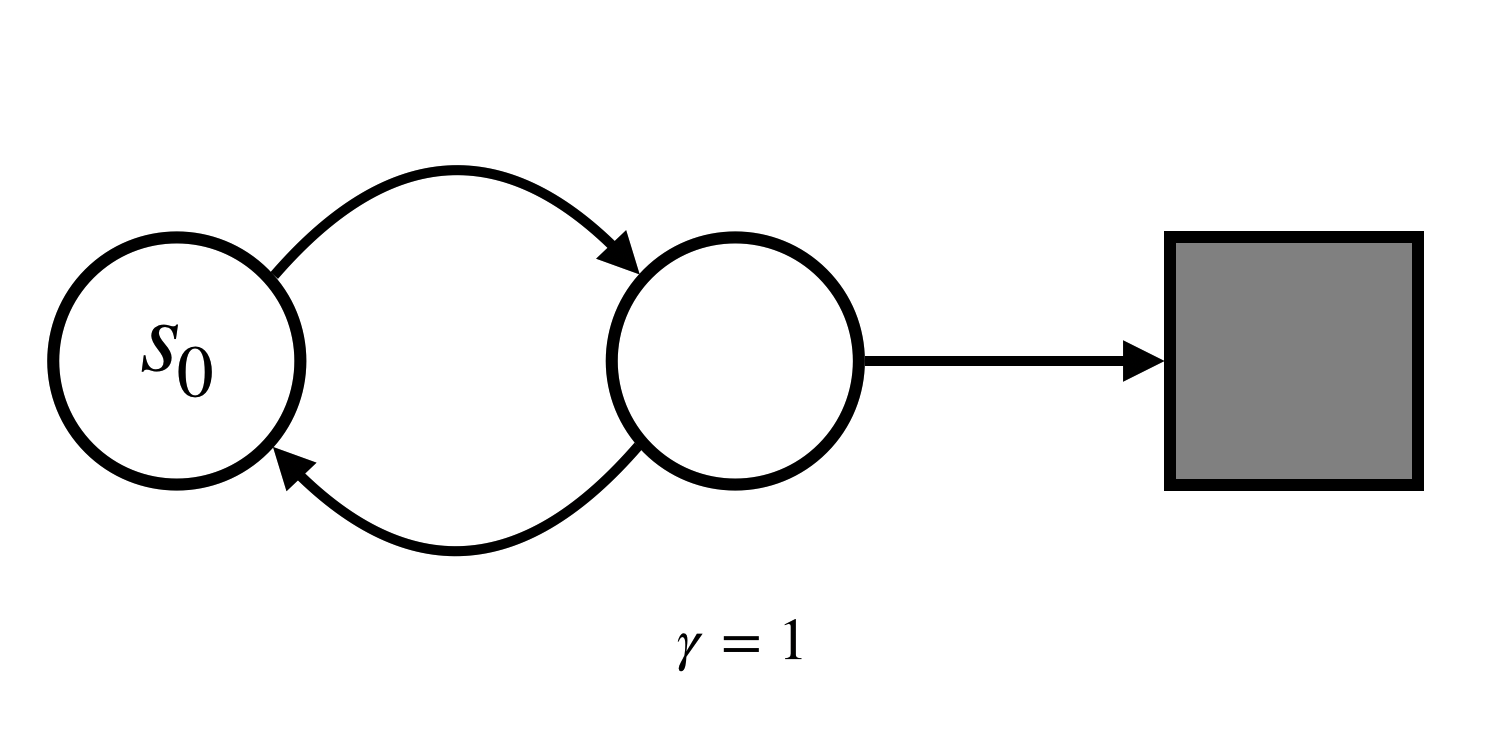
\includegraphics[width=0.5\textwidth]{mdp_episodic}
    \caption{An undiscounted episodic task specified using terminal states on a small MDP. Rewards are omitted for clarity.}
    \label{fig:mdp_episodic}
\end{figure}

Here, $s_0$ denotes a starting state, and a square denotes a terminal state. By allowing state-dependent discounting, a terminal state can equivalently be specified as a state with $\gamma(s) = 0$ and a transition back to a starting state. An MDP with state-dependent discounting which specifies an equivalent undiscounted episodic task can be seen in Figure \ref{fig:mdp_continuing}.

\begin{figure}[H]
    \centering
    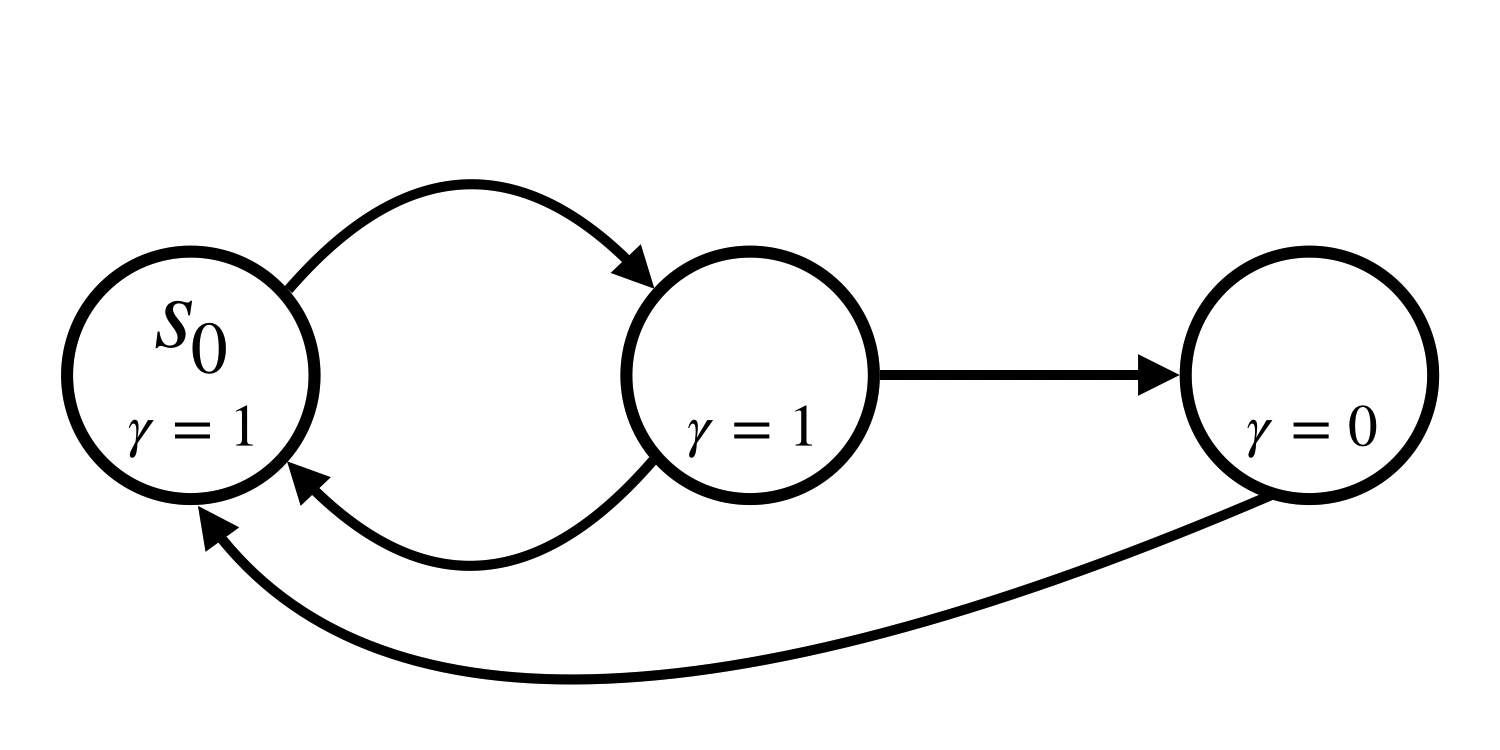
\includegraphics[width=0.5\textwidth]{mdp_continuing}
    \caption{An undiscounted episodic task specified as a continuing task with state-dependent discounting. Rewards are omitted for clarity.}
    \label{fig:mdp_continuing}
\end{figure}

Under state-dependent discounting, a future reward is now weighted by the product of discount rates between a time-step and that of when the reward occurs:

\begin{equation}
    G_t = \sum_{k=0}^{\infty}{R_{t+k+1}\prod_{i=1}^{k}{\gamma(S_{t+i})}}
    \label{eqn:prodreturn}
\end{equation}

Based on this, it's evident that the infinite sum is well defined in a continuing setting even with momentary $\gamma(s) \geq 1$, as long as the product of discount rates is 0 in the limit w.p.1.

\section{Programming Examples}

The following subsections contain code for evaluating an equiprobable random policy on the two state MDP detailed in Figure \ref{fig:twostatemdp}. The first estimates it by simulating the policy from each state for some number of steps, and averages the sampled returns into each state's value estimate. The second directly solves the Bellman equation as a linear system of equations.

\newpage
\begin{figure}[h]
    \centering
    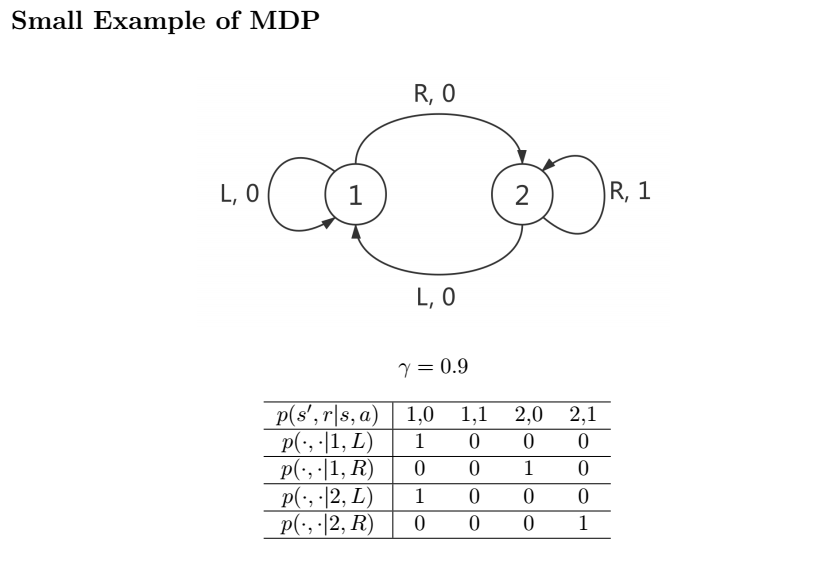
\includegraphics[width=1.0\textwidth]{twostatemdp_diagram}
    \caption{Diagram of the two-state MDP used in the programming examples}
    \label{fig:twostatemdp}
\end{figure}

\newpage
\subsection{Monte Carlo Simulation}
\lstset{frame=lines}
\lstinputlisting[language=python]{twostatemdp_montecarlosim.py}

\newpage
\subsection{Solving a Linear System}
\lstset{frame=lines}
\lstinputlisting[language=python]{twostatemdp_linearsystem.py}
\end{document}
